\documentclass[aspectratio=169]{beamer}
\usepackage[utf8]{inputenc}
\usepackage{booktabs}
\usepackage{graphicx}
\usepackage{amsmath}
\usepackage{tikz}

\usetheme{default}
\definecolor{iitblue}{RGB}{15,58,92}
\setbeamercolor{structure}{fg=iitblue}
\setbeamercolor{frametitle}{bg=iitblue,fg=white}
\setbeamercolor{title}{fg=iitblue}
\setbeamerfont{frametitle}{series=\bfseries}
\setbeamertemplate{navigation symbols}{}
\setbeamertemplate{footline}{%
  \leavevmode
  \hbox{\begin{beamercolorbox}[wd=1\paperwidth,ht=2.7ex,dp=1ex,leftskip=1em,rightskip=1em]{iitblue}
  \usebeamercolor[fg]{structure}\color{white}\scriptsize
  Department of Physics, Indian Institute of Technology, Bhubaneswar
  \hfill \insertframenumber
  \end{beamercolorbox}}%
}
\setbeamertemplate{itemize item}{\color{iitblue}\textbullet}
\setbeamertemplate{itemize subitem}{\color{iitblue}\textendash}

\title{\textbf{Do the Quantum Parts Help?\\[2pt]\large A Component-Wise Ablation of the Hamiltonian Vision Kernel}}
\author{Sparsho Chakraborty}
\institute{Department of Physics, Indian Institute of Technology, Bhubaneswar}
\date{July 14, 2026}

\begin{document}

% ---------- Slide 1: Title ----------
\begin{frame}
\titlepage
\end{frame}

% ---------- Slide 2: Overview ----------
\begin{frame}{Overview}
\begin{enumerate}
  \item Motivation
  \item HVK Pipeline (recap)
  \item Evaluation Protocol
  \item Results: Component Ablation
  \item Results: Held-Out Real Images
  \item The Leakage Lesson
  \item Scoped Positive Results
  \item Conclusion
\end{enumerate}
\end{frame}

% ---------- Slide 3: Motivation ----------
\begin{frame}{Motivation}
\begin{itemize}
  \item Hybrid quantum--classical vision models routinely claim an advantage over classical baselines.
  \item Rarely isolated: \textbf{which component} is actually responsible?
  \item Rarely matched: classical control parameter budget vs.\ quantum model.
  \item Rarely audited: same-set fit vs.\ held-out generalization; target--feature leakage.
\end{itemize}
\vfill
\begin{block}{Question}
Does \emph{any} quantum component of HVK do measurable work on real, held-out images?
\end{block}
\end{frame}

% ---------- Slide 4: Model Pipeline (KEPT UNCHANGED) ----------
\begin{frame}[plain]
\begin{tikzpicture}[remember picture, overlay]
\node[at=(current page.center)] {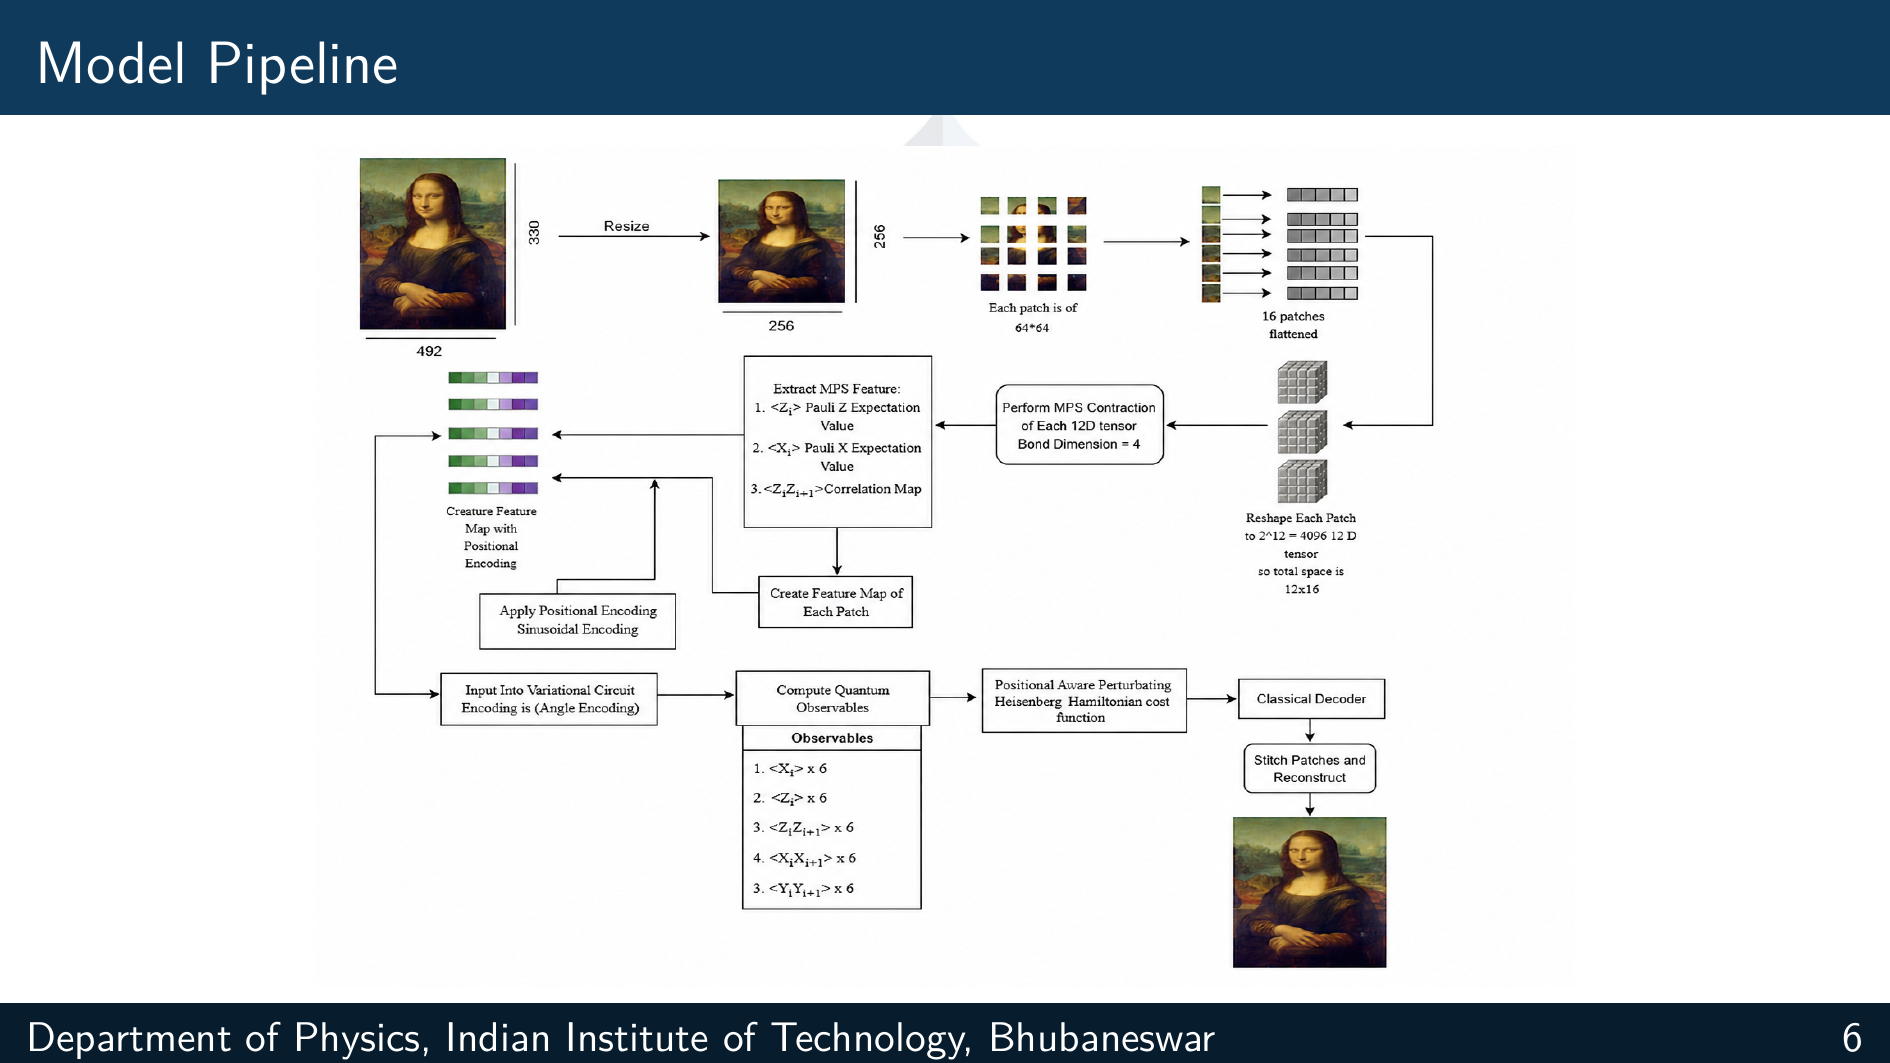
\includegraphics[width=\paperwidth,height=\paperheight]{figures/kept_model_pipeline-06.png}};
\end{tikzpicture}
\end{frame}

% ---------- Slide 5: Positional Encoding / Image Preparation (KEPT UNCHANGED) ----------
\begin{frame}[plain]
\begin{tikzpicture}[remember picture, overlay]
\node[at=(current page.center)] {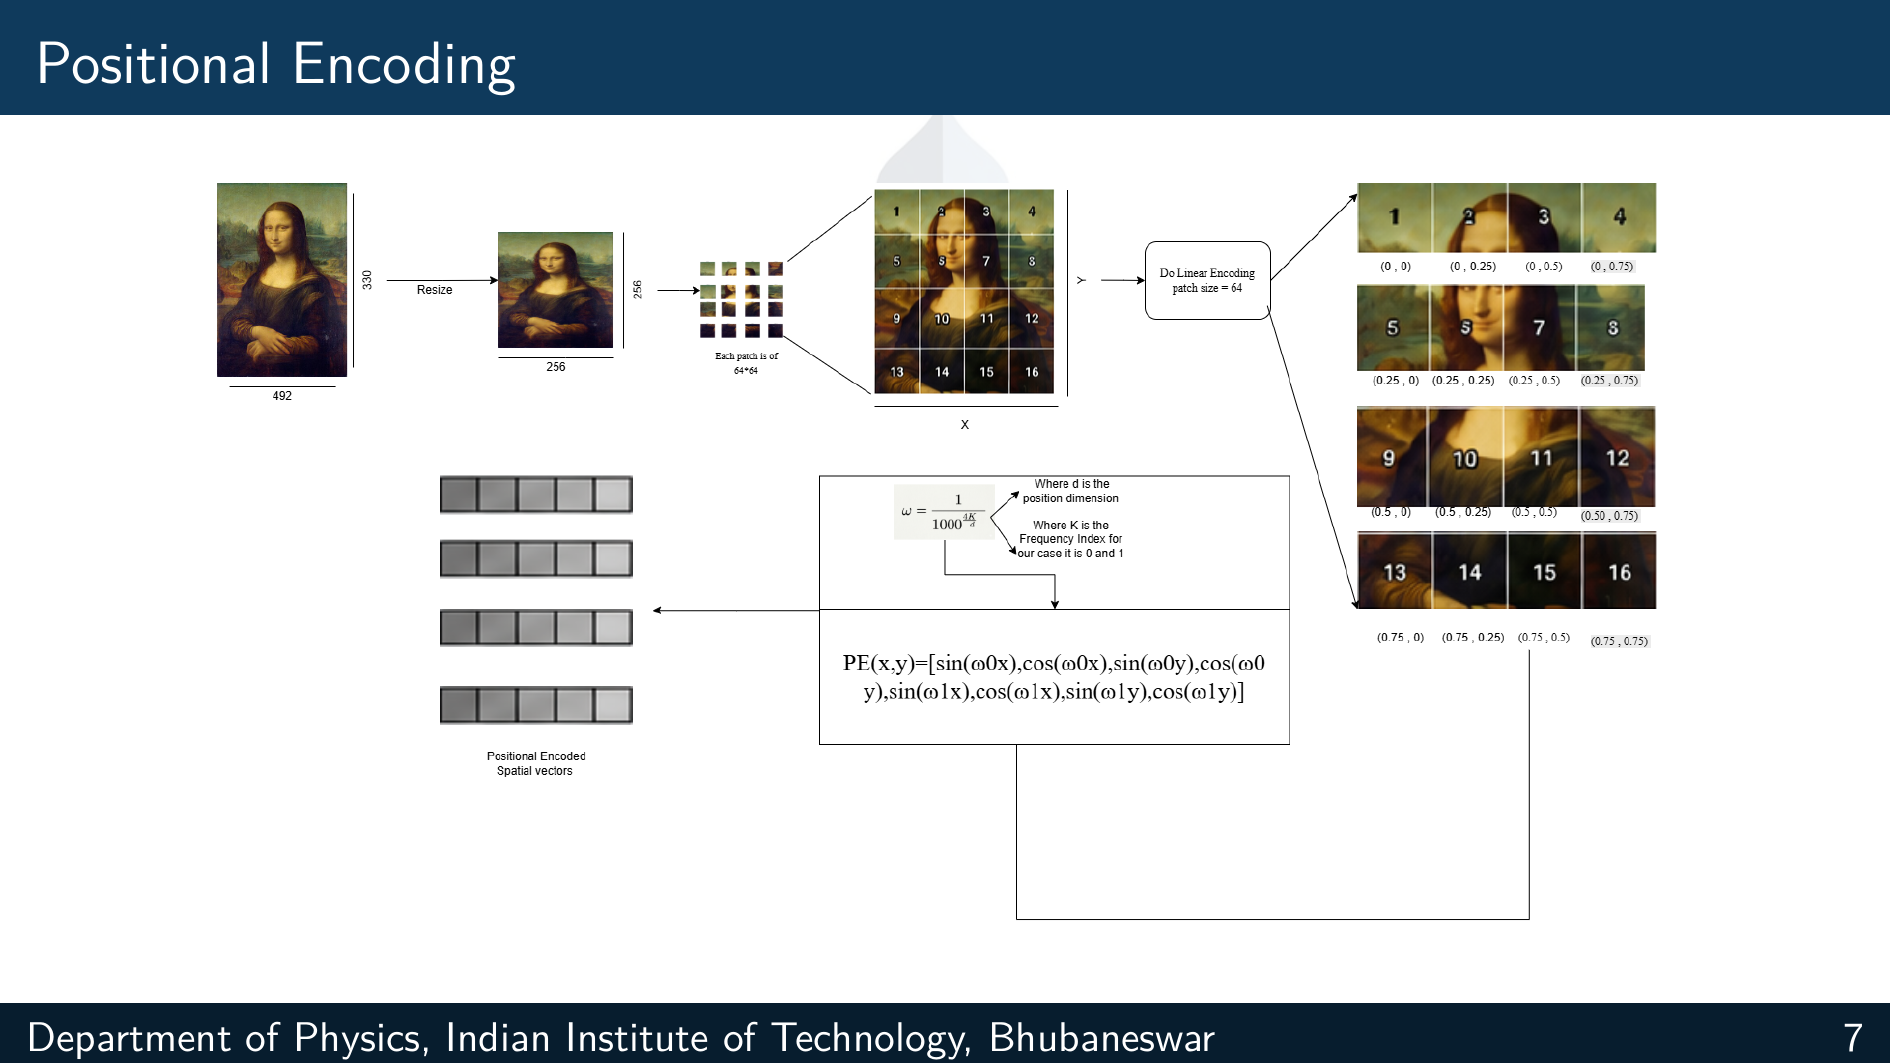
\includegraphics[width=\paperwidth,height=\paperheight]{figures/kept_positional_encoding-07.png}};
\end{tikzpicture}
\end{frame}

% ---------- Slide 6: Evaluation Protocol ----------
\begin{frame}{Evaluation Protocol}
\begin{itemize}
  \item \textbf{Freeze isolation:} train only classical decoder, or only quantum circuit.
  \item \textbf{Resource-matched controls:} same feature width, same readout parameter count.
  \item \textbf{Leakage audit:} target must not be linearly recoverable from a model's own input features.
  \item \textbf{Multi-seed statistics:} 5 seeds, paired Wilcoxon test, bootstrap 95\% CI.
  \item \textbf{Held-out $\neq$ same-set:} generalization claims require held-out splits only.
\end{itemize}
\end{frame}

% ---------- Slide 7: Component Ablation Table ----------
\begin{frame}{Which Component Is Load-Bearing? (Monalisa, 5 seeds)}
\centering
\scriptsize
\begin{tabular}{lccc}
\toprule
Variant & PSNR (dB) & $\Delta$PSNR & Verdict \\
\midrule
Freeze classical, train quantum & $10.93\pm0.00$ & $-22.03$ & Collapses \\
Random VQC output & $27.96\pm0.28$ & $-5.01$ & Much worse \\
Shared VQC baseline & $32.97\pm0.22$ & $0.00$ & Reference \\
No entanglement & $32.98\pm0.15$ & $+0.02$ & Not significant \\
No MPS & $33.04\pm0.15$ & $+0.08$ & Not significant \\
Freeze quantum, train classical & $33.26\pm0.10$ & $+0.30$ & Ties baseline \\
Parameter-matched classical & $33.37\pm0.08$ & $+0.40$ & Exceeds baseline \\
No energy loss & $33.40\pm0.06$ & $+0.44$ & Exceeds baseline \\
Classical tanh replacement & $33.50\pm0.00$ & $+0.54$ & Exceeds baseline \\
\bottomrule
\end{tabular}
\vspace{6pt}
\begin{block}{}
\centering \textbf{The classical decoder is load-bearing. The quantum circuit is not.}
\end{block}
\end{frame}

% ---------- Slide 8: Held-out CIFAR-10 headline result ----------
\begin{frame}{Headline Result: Held-Out CIFAR-10}
\begin{columns}[T]
\begin{column}{0.5\textwidth}
\centering\scriptsize
\begin{tabular}{lc}
\toprule
Model & PSNR (dB) \\
\midrule
Local observables / raw-linear & $18.80\pm1.42$ \\
ZZ-only observables & $18.56\pm1.49$ \\
No entanglement & $18.46\pm1.32$ \\
\textbf{HVK2D (trained)} & $\mathbf{18.12\pm1.54}$ \\
Random VQC & $11.15\pm1.19$ \\
\bottomrule
\end{tabular}
\vspace{4pt}
{\tiny Paired Wilcoxon vs.\ raw-linear: $p=9.5\times10^{-6}$, $n=20$}
\end{column}
\begin{column}{0.5\textwidth}
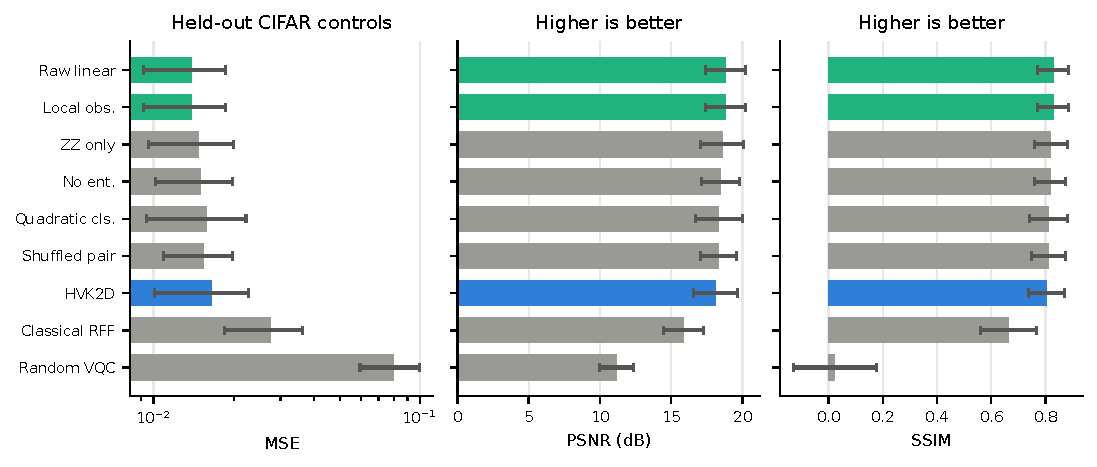
\includegraphics[width=\linewidth]{figures/real_cifar_holdout_summary.pdf}
\end{column}
\end{columns}
\vspace{4pt}
\centering\textbf{Every quantum ablation ties or beats trained HVK2D on held-out images.}
\end{frame}

% ---------- Slide 9: Multi-dataset generalization ----------
\begin{frame}{Same Pattern Across Six Datasets}
\centering\scriptsize
\begin{tabular}{lccc}
\toprule
Dataset & Best local/raw & HVK2D pair & Winner \\
\midrule
CIFAR-10 (native) & $21.17\pm1.98$ & $19.99\pm2.02$ & Local/raw \\
MNIST & $16.55\pm1.27$ & $16.12\pm1.34$ & Local/raw \\
Fashion-MNIST & $17.67\pm1.71$ & $17.33\pm1.80$ & Local/raw \\
PathMNIST & $27.52\pm6.02$ & $27.01\pm5.81$ & Local/raw \\
BloodMNIST & $24.79\pm1.78$ & $24.24\pm1.66$ & Local/raw \\
PneumoniaMNIST & $26.49\pm2.48$ & $25.73\pm2.29$ & Local/raw \\
\bottomrule
\end{tabular}
\vspace{8pt}

\centering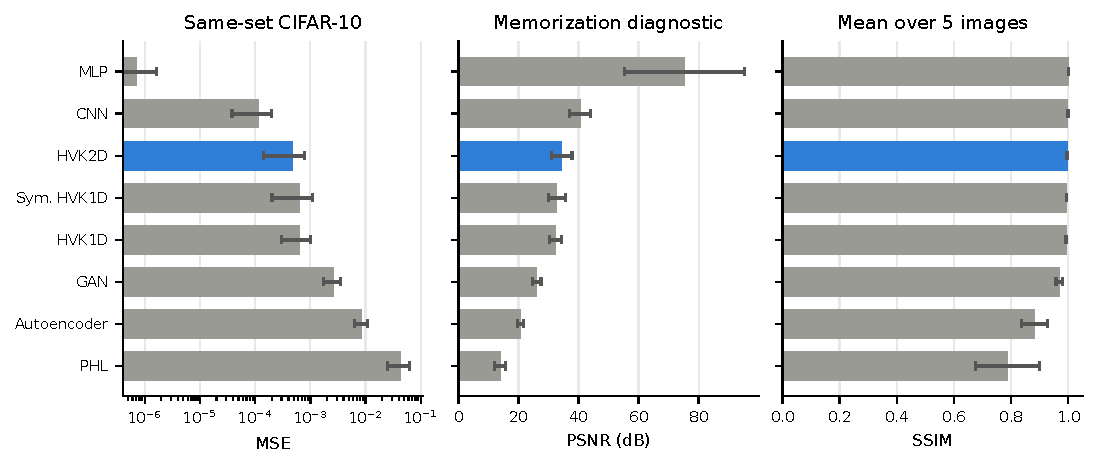
\includegraphics[width=0.55\linewidth]{figures/cifar_metric_comparison.pdf}
\end{frame}

% ---------- Slide 10: The Leakage Lesson ----------
\begin{frame}{A Circular Benchmark --- and How We Caught It}
\begin{itemize}
  \item An earlier diagnostic reported $R^2 = 1.0000$, PSNR $= 120$~dB for the entangling model.
  \item Cause: the target was built from the \textbf{same product terms} handed to the model as input features.
  \item The model was copying, not learning. Withdrawn from every claim in the paper.
\end{itemize}
\vspace{6pt}
\begin{block}{Reusable rule}
Before trusting a favorable diagnostic: verify the target is \emph{not} linearly recoverable from a candidate's own input features.
\end{block}
\end{frame}

% ---------- Slide 11: Scoped positive results ----------
\begin{frame}{Two Narrow, Honest Positive Results}
\begin{columns}[T]
\begin{column}{0.5\textwidth}
\centering\scriptsize
\textbf{Entanglement-necessity}\\[2pt]
\begin{tabular}{lc}
\toprule
Model & $R^2$ \\
\midrule
HVK2D entangling & $0.974$ \\
No entanglement & $0.019$ \\
Random VQC & $-0.173$ \\
\bottomrule
\end{tabular}
\vspace{4pt}
{\tiny Deliberately favorable, leakage-audited synthetic target.}
\end{column}
\begin{column}{0.5\textwidth}
\centering\scriptsize
\textbf{$D_4$ symmetry (provable)}\\[2pt]
\begin{tabular}{lc}
\toprule
Map & Equiv. error \\
\midrule
$D_4$-pooled HVK2D & $9.6\times10^{-17}$ \\
HVK2D positional & $0.815$ \\
Local/raw & $0.837$ \\
\bottomrule
\end{tabular}
\vspace{4pt}
{\tiny Verified over 7000 patch transforms.}
\end{column}
\end{columns}
\vspace{6pt}
\centering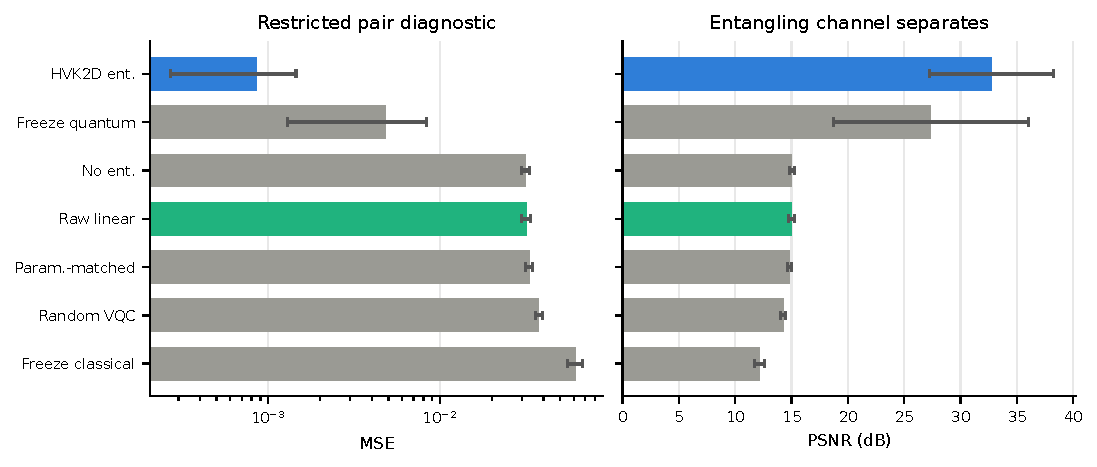
\includegraphics[width=0.5\linewidth]{figures/full_ablation_metric_comparison.pdf}
\end{frame}

% ---------- Slide 12: Guidelines ----------
\begin{frame}{Guidelines for Evaluating Hybrid Quantum--Classical Vision Models}
\begin{enumerate}
  \item Resource-match every classical control.
  \item Freeze-isolate each trainable component.
  \item Audit every favorable diagnostic for target--feature leakage.
  \item Report held-out, not same-set, performance as primary evidence.
  \item Report multiple seeds with error bars.
\end{enumerate}
\end{frame}

% ---------- Slide 13: Conclusion ----------
\begin{frame}{Conclusion}
\begin{itemize}
  \item On held-out real images, \textbf{no quantum component of HVK is load-bearing} --- classical controls tie or win.
  \item The classical decoder, not the quantum circuit, does the work.
  \item Entanglement helps only in a narrow, leakage-audited, pair-correlation setting.
  \item $D_4$-pooling gives a provable symmetry guarantee, independent of any advantage claim.
\end{itemize}
\vspace{6pt}
\centering\textit{The contribution is the evaluation protocol itself.}
\end{frame}

% ---------- Slide 14: Thank you ----------
\begin{frame}[plain]
\begin{center}
\vspace{2cm}
{\Huge \textbf{THANK YOU!}}
\vspace{1cm}


\includegraphics[width=2cm]{figures/iitbbslogo.png}
\end{center}
\end{frame}

\end{document}
